\chapter{Verwendete Technologien} \label{technologien}

\section{\LaTeX}
Diese Diplomarbeit wurde mit \LaTeX \space (\textit{{\bf{\textit{La}}}mport {\bf{\textit{\TeX}}}}) verfasst. Dieses Softwarepaket stellt eine Bibliothek von \TeX-Makros dar. \LaTeX \space ist plattformunabhängig und eine gute Möglichkeit gegenüber anderen Textverarbeitungsprogrammen. Dieses Softwarepaket funktioniert nach dem WYSIWYAF-Prinzip (\textit{{\bf{W}}hat {\bf{y}}ou {\bf{s}}ee {\bf{i}}s {\bf{w}}hat {\bf{y}}ou {\bf{a}}sked {\bf{f}}or}), das bedeutet es wird in normalen Textdateien mit Befehlen gearbeitet, die dann in verschiedene Formate (PDF, DVI, PostScript) kompiliert werden können. \autocite{wikiLatex}

\section{BibTeX}
BibTeX erstellt in \LaTeX-Dokumenten Literaturangaben und -Verzeichnisse. Dafür wird eine Literaturdatenbank, ein Textdokument mit der Endung .bib, erstellt, wo jedes Buch, Webseite oder Werk nach einer bestimmten Syntax hineingeschrieben wird. Zur Erstellung eines Verzeichnisses werden aus dem \LaTeX-Dokument alle Zitatverweise herausgesucht und mit der Literaturdatenbank zu einem Werk zugewiesen. Das Verzeichnis wird somit automatisch nach dem eingestellten Stil erstellt. \autocite{wikiBibtex}

\section{TeXstudio}
Die \LaTeX-Dokumente dieser Diplomarbeit wurden mit TeXstudio erstellt. Dieser Editor ist plattformunabhängig und er stößt die Kompilierung an und zeigt Dokumente an. Es besitzt eine Autocomplete-Funktion für \LaTeX-Befehle, Echtzeit-Syntaxkontrolle und -Rechtschreibüberprüfung. Weiteres besteht die Möglichkeit, dass Unicode-kodierte Dateien verarbeitet werden. \autocite{wikiTexstudio}

\section{.NET Core 3.1 und C\#}
Für das Backend der Diplomarbeit wurde das Microsoft .NET Framework .NET Core 3.1 verwendet. Die Anwendungen wurden mit der objektorientierten Programmiersprache C\#  erstellt. \autocite{wikiDotnet}

\subsection{.NET Core 3.1}
.NET Core wurde 2015 als Abzweigung vom .NET Framework vorgestellt. Es wurde für eine bessere Modularität und eine leichtere Portierbarkeit auf Microsoft-fremde Plattformen entwickelt. 2016 wurde angekündigt, dass .NET Core mit mehreren APIs ausgestattet wird, um die Kompatibilität zwischen verschiedenen .NET Frameworks zu verbessern. \autocite{wikiDotnet} \\
.NET Core 3.1 wurde am 03.12.2019 als Nachfolger von der Version 2.2 veröffentlicht. Dieses Framework unterstützt die Programmiersprachen C\#, F\#, C++/CLI und Visual Basic .NET. \autocite{wikiDotnetCore}

\subsection{C\#}
C\# wurde von Microsoft entwickelt und 2001 veröffentlicht. Diese plattformunabhängige, objektorientierte Programmiersprache basiert auf Konzepten von den Programmiersprachen Delphi, C, Haskell, C++ und Java.
C\# wird meist nicht gleich von den Compiler in die Maschinensprache, sondern in die Zwischensprache Common Intermediate Language (CIL) übersetzt. Im Listing \ref{lst:cSharpSyntax} sieht man ein Syntaxbeispiel con C\#. Die Methode \texttt{Main} in der Klasse \texttt{Program} schreibt beim Aufruf "Hello World!" auf die Konsole. \autocite{wikiCSharp}

\begin{lstlisting}[caption={C\#-Syntaxbeispiel}, language={[Sharp]C},label={lst:cSharpSyntax}]
	using System;
	namespace HelloWorld
	{
		public class Program
		{
			public static void Main(string[] args)
			{
				Console.WriteLine("Hello World!");
			}
		}
	}
\end{lstlisting}
\section{Angular}
Das Frontend dieser Diplomarbeit wurde mit den Webapplikationsframework Angular geschrieben. Angular ist ein Open-Source-Software, basiert auf TypeScript und wird von einer Online-Community und Google LLC entwickelt.\\
Das Architekturkonzept von Angular ist eine Hierarchie von Komponenten. Durch Module wird Code schneller und Funktionalitäten können ausgelagert werden. TypeScript wird als Entwicklungssprache empfohlen, da diese Generics, statische Typisierung und klassenbasierte objektorientierte Programmierung ermöglicht. \autocite{wikiAngular}
Weiters bietet Angular:

\begin{itemize}
	\item Reaktive Programmierung mit RxJs
	\item Einfaches Routing
	\item Asynchrone Kompilierung von Templates
	\item Dynamisches Laden
	\item Dependency Injection
	\item Lazy- \& Eagerloading
\end{itemize}

\section{TypeScript}
TypeScript wurde von Microsoft entwickelt und 2012 veröffentlicht. Diese Programmiersprache basiert auf den ECMAScript6-Standard. Der TypeScript-Compiler kompliliert den Code in plain-JavaScript, deshalb ist jeder JavaScript-Code auch ein gültiger TypeScript-Code. Somit sind Bibliotheken wie jQuery oder Angular 1 auch in TypeScript verwendbar. \autocite{wikiTypeScript} \\

TypeScript bietet viele unterstützende Features:

\begin{itemize}
	\item Klassen
	\item Module
	\item Arrow-Syntax für anonyme Funktionen
	\item Optionale Parameter und Standardparameter
	\item Namensräume
	\item Tupel
	\item Async/Await
	\item Generische Programmierung
	\item Aufzählungstyp
	\item Interfaces
	\item Type Erasure
	\item Typinferenz
	\item Methodensignatur
	\item Enums
\end{itemize}

\begin{lstlisting}[caption={TypeScript-Beispiel Function}, language=JavaScript]
	public add(a: number, b: number): number {
		return a + b;
	}
\end{lstlisting}

\begin{lstlisting}[caption={TypeScript-Beispiel Klasse},captionpos=b, language=JavaScript]
	class Person {
		private name: string;
		private age: number;
		private salary: number;
		
		constructor(name: string, age: number, salary: number) {
			this.name = name;
			this.age = age;
			this.salary = salary;
		}
		
		toString(): string {
			return `${this.name} (${this.age}): (${this.salary})`;
		}
	}
\end{lstlisting}
\begin{lstlisting}[caption={TypeScript-Beispiel Generische Programmierung}, language=JavaScript]
	function doSomething<T>(arg: T): T {
		return arg;
	}
\end{lstlisting}

\section{Visual Studio Code}
Das Frontend dieser Diplomarbeit wurde in Visual Studio Code programmiert. Dieser Quelltexteditor erschien 2015 von Microsoft und arbeitet mit Quelldateien und Ordnern in Workspaces. Es bietet Versionsverwaltung, Autovervollständigung, Debugging und Syntaxhervorhebung. Es unterstützt Programmiersprachen wie Java, C++, C\#, JavaScript, TypeScript, Python und viele mehr. Für Visual Studio Code gibt es Plug-ins, die das programmieren sehr vereinfachen können. \autocite{wikiVisualStudioCode}

\begin{figure}[H]
	\centerline{
		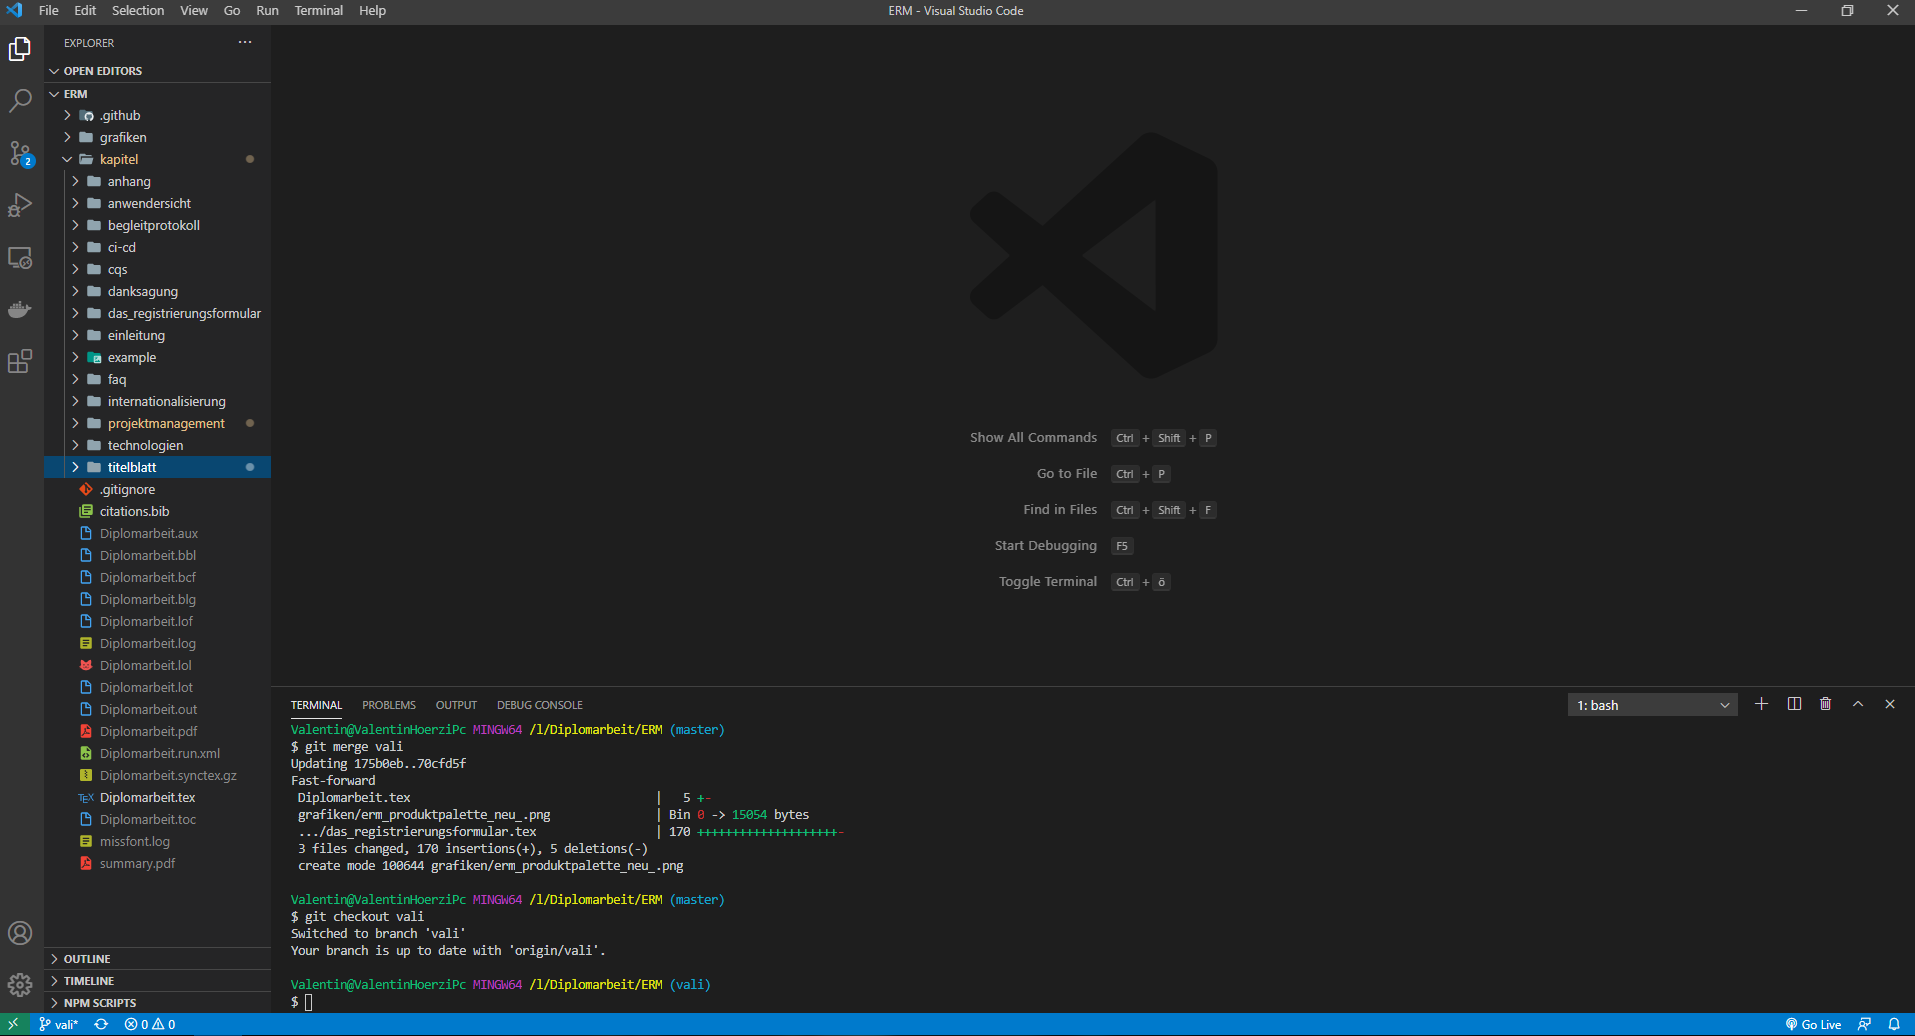
\includegraphics[width=1\textwidth, frame]{./grafiken/vs_code_startbildschirm.PNG}
	}
	\vskip0pt
	\caption{UI von Visual Studio Code} \label{fig:visualStudioCodeStartview}
\end{figure}

\section{Visual Studio 2019}
%Das Backend dieser Diplomarbeit wurde im Visual Studio programmiert. Die von Microsoft stammende Entwicklungsumgebung ist 1997 erschienen und arbeitet mit Projektdateien. Visual Studio bietet viele Funktionen wie IntelliSense, automatische Syntaxprüfung, Debugger mit Bearbeiten und Fortfahren und vieles mehr. Seit 2005 hat es einen integrierten Webserver. Es unterstützt einige Programmiersprachen, wie C\#, C++, C, Visual Basic .NET, TypeScript und viele mehr. \autocite{wikiVisualStudio}

Für das Backend der Diplomarbeit wurde Microsoft Visual Studio gewählt. Diese IDE (Integrated Development Environment) unterstützt den Programmierer durch eine ausgereifte Entwicklungsumgebung mit vielen Features.\\

Am nachfolgenden Screenshot sieht man den Startbildschirm von Microsoft Visual Studio 2019
\begin{figure}[h]
	\centerline{
		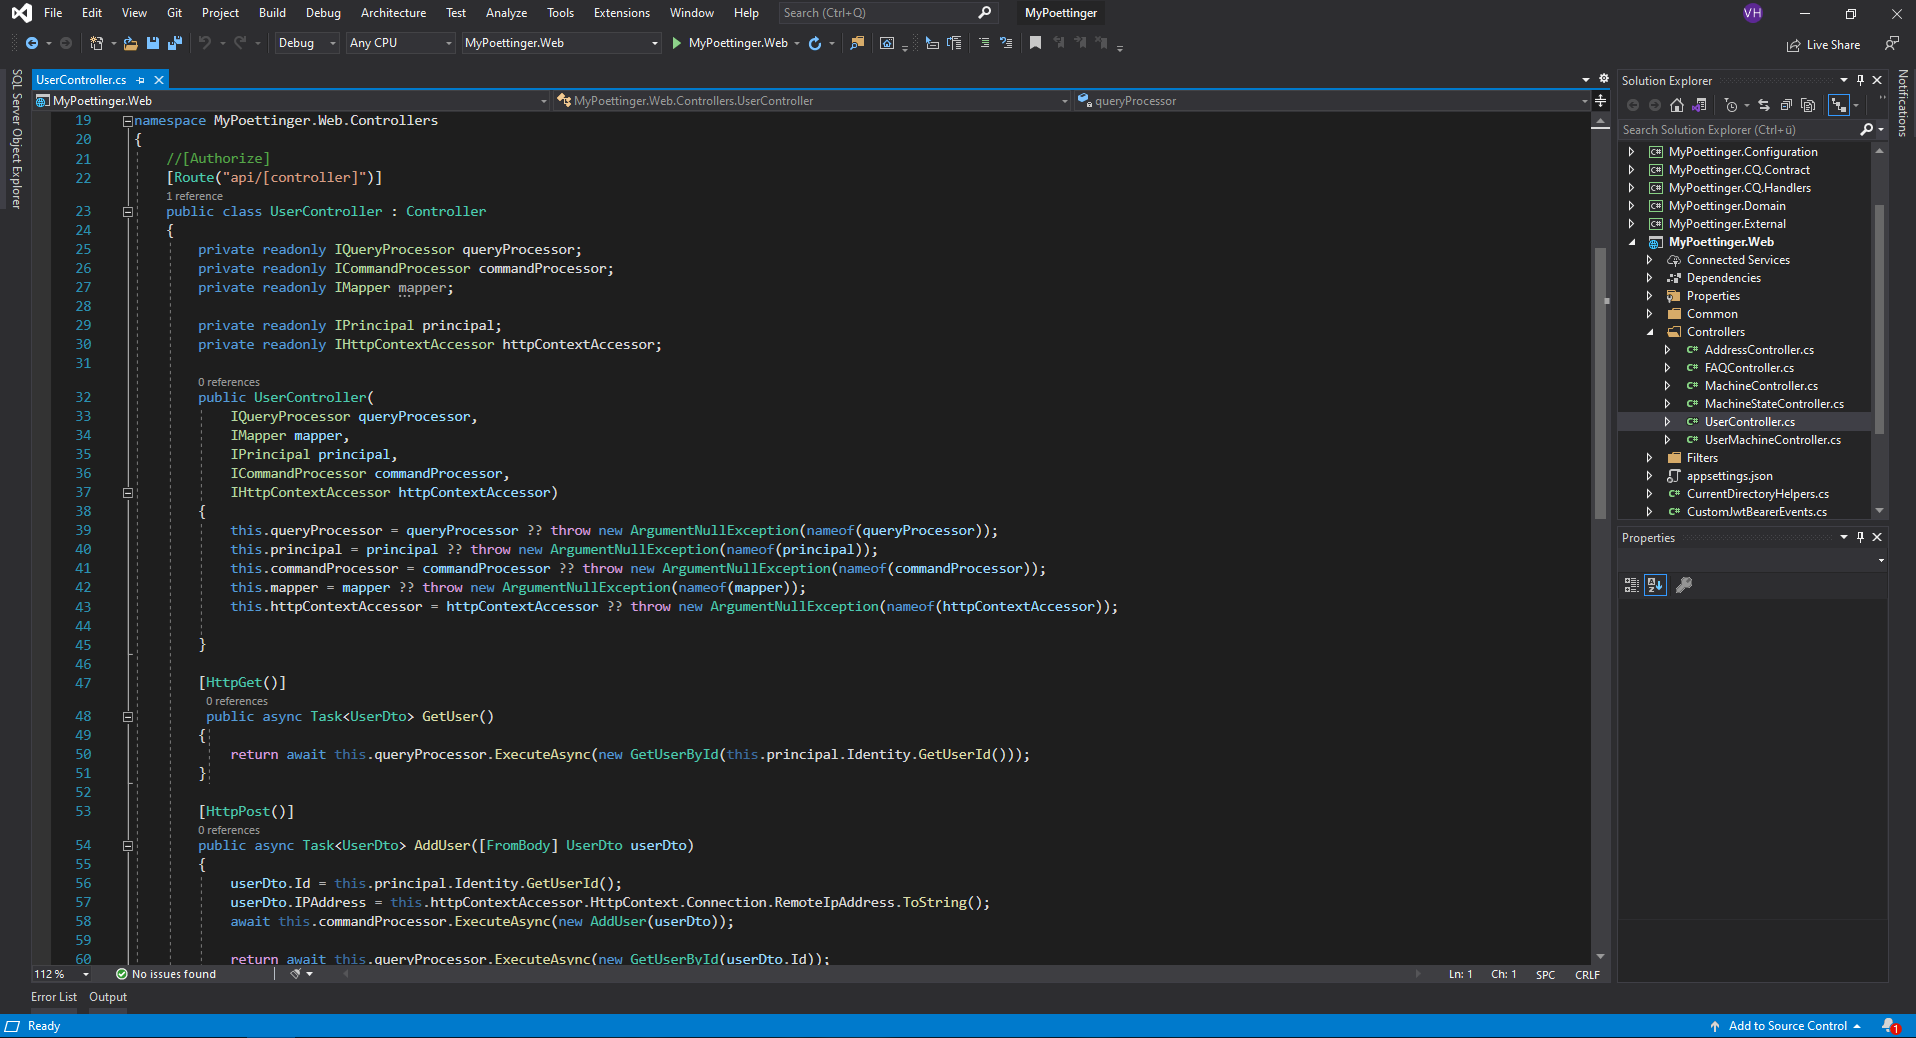
\includegraphics[width=1\textwidth, frame]{./grafiken/visual_studio_startview.png}
	}
	\vskip0pt
	\caption{UI von Microsoft Visual Studio 2019} \label{fig:visualStudioStartview}
\end{figure}

Es gibt folgende Editionen von Microsoft Visual Studio 2019, wobei sie sich in den vorhandenen Funktionen unterscheiden:
\begin{itemize}
	\item Community Edition
	\item Professional Edition
	\item Test Professional Edition
	\item Enterprise Edition
\end{itemize}

Diese Diplomarbeit wurde mit der Community Edition erstellt, da diese Version alles zur Verfügung stellt, was gebraucht wurde. \autocite{wikiVisualStudio}

Laut \autocite{wikiVisualStudio} bietet Microsoft Visual Studio 2019 viele unterstützende Features:

\begin{itemize}
	\item Online-Hilfe, die von der Cursorposition abhängig ist
	\item Ein- und Ausblenden von Codeblöcken
	\item Server-Explorer zum Zugriff auf Datenquellen
	\item Automatische Syntaxprüfung und IntelliSense
	\item Automatische Methoden- und Funktionsergänzung während der Quelltext-Eingabe
	\item Einbindung von Web Services
	\item ActiveX- und .NET-Bibliotheken
	\item Farbliche Kennung von Schlüsselwörtern
	\item Integrierter Debugger mit der Bearbeiten-und-Fortfahren-Funktion
	\item Windows-Nachrichtendienst
	\item WYSIWYG-Editoren zur Benutzeroberflächenentwicklung
\end{itemize}
\section{Git Versionsverwaltung}
Git wurde 2005 veröffentlicht. Diese Software dient zur verteilten Versionsverwaltung von Dateien. Wichtige Bestandteile von Git sind die Erstellung neuer Entwicklungszweige, den sogenannten Branches und das Zusammenführen von zwei Zweigen. Da es keinen zentralen Server gibt, besitzt jeder Benutzer das gesamte Repository als Kopie lokal. Dadurch benötigt man für fast alle Aktionen keinen Internetzugriff. Mit den Hash-Wert eines Commites wird die History eines Projektes gespeichert. Durch diese Speicherung ist die History gesichert, da es nicht möglich ist, einen Commit zu verändern, der dann den selben Hash-Wert hat. \autocite{wikiGit}

\subsection{GitHub}
Für das Diplomarbeitsdokument wurde GitHub verwendet. GitHub wurde 2008 veröffentlicht und gehört seit 2018 zu Microsoft. Es dient zur Versionsverwaltung von Projekten. Diese Open-Source-Software ermöglicht ein leichtes Branching, Merging und Commiting für alle Entwickler. \autocite{wikiGitHub}

\begin{figure}[H]
	\centerline{
		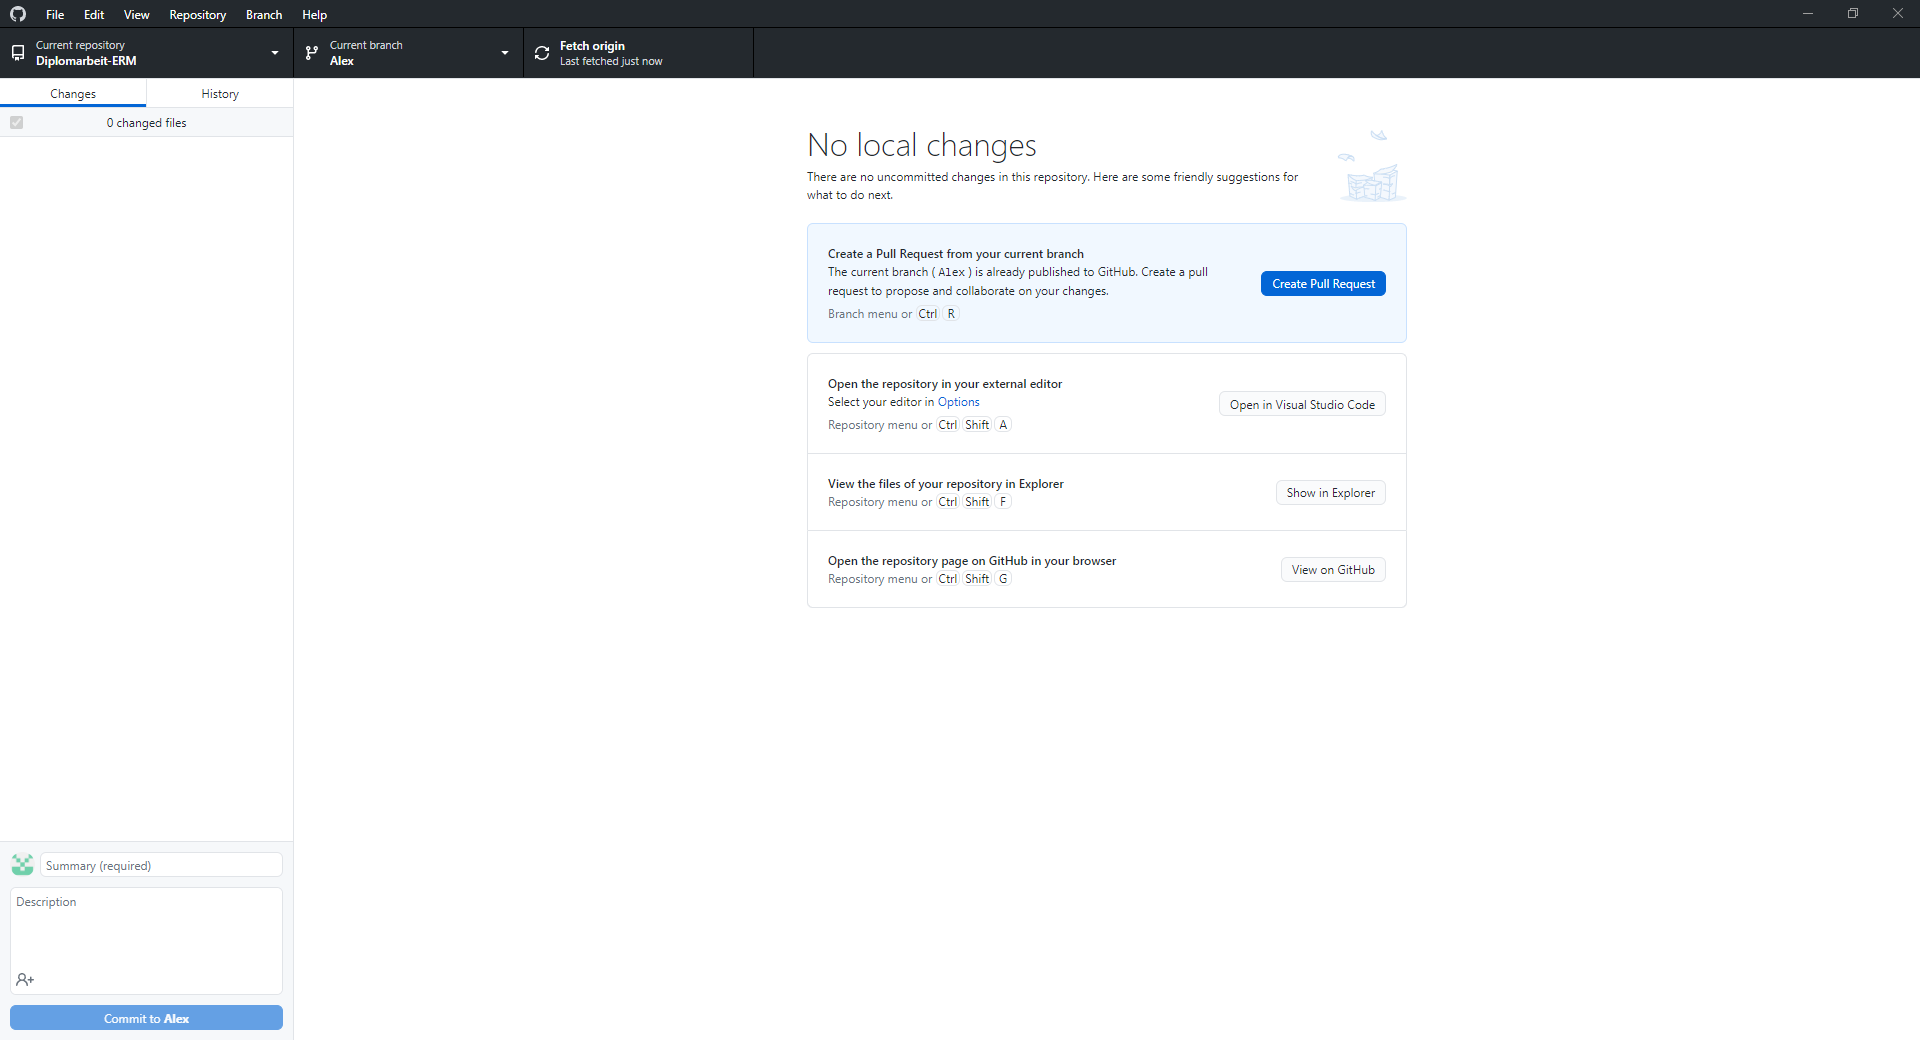
\includegraphics[width=1\textwidth, frame]{./grafiken/github_screen.png}
	}
	\vskip0pt
	\caption{UI von GitHub} \label{fig:github}
\end{figure}

\subsection{GitLab}
Für das Projekt der Diplomarbeit wurde GitLab verwendet. Die Versionsverwaltung basiert auf Git und ist eine Webanwendung. Weitere Features von GitLab ist ein Issue-Tracking-System mit einem Kanban-Board, ein Continuous Integration und Continuous Delivery System, eine Projekt-Wiki, eine Container-Registry und eine Multi-Cluster-Verwaltung. GitLab ist eine Open-Source-Software und wird als Software as a Service angeboten. \autocite{wikiGitLab}

\begin{figure}[H]
	\centerline{
		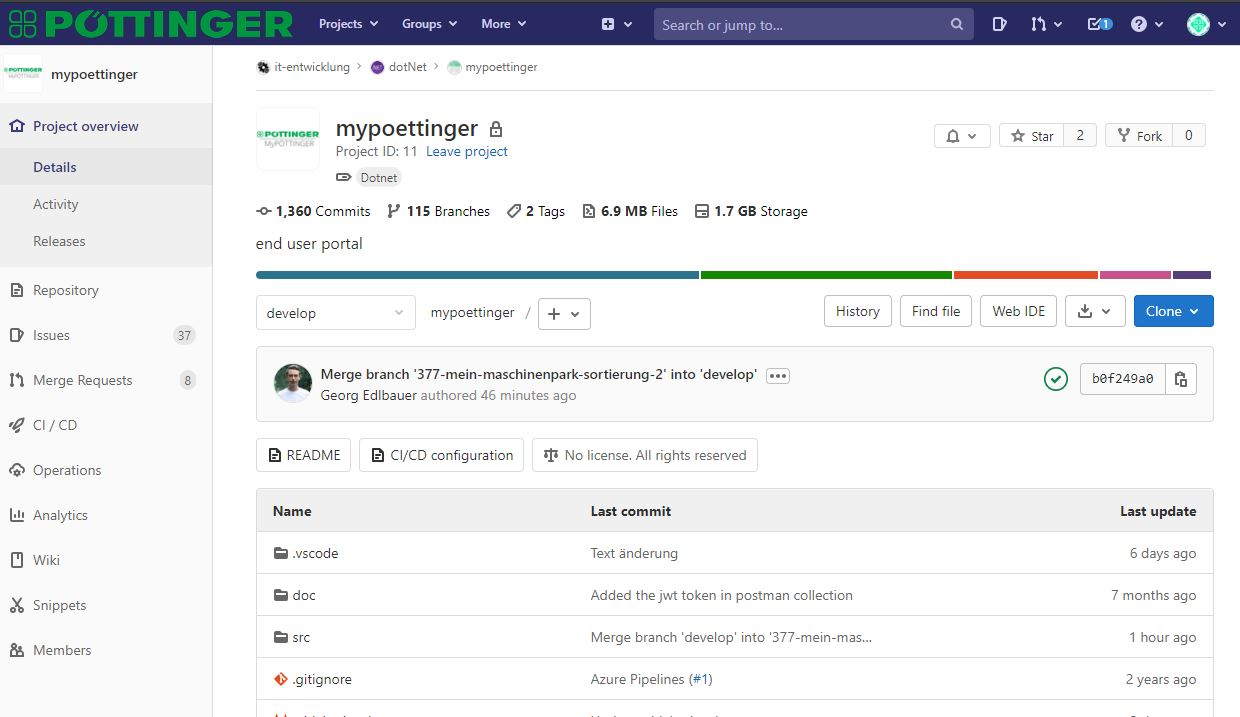
\includegraphics[width=1\textwidth, frame]{./grafiken/gitlab_startseite.JPG}
	}
	\vskip0pt
	\caption{UI von GitLab}
\end{figure}
\section{Postman}
Um die APIs (application programming interface) des Backendes der Diplomarbeit zu testen, wurde Postman verwendet. Postman bietet die Funktion, Http-Requests an jede beliebige URL mit jeder verfügbaren HTTP-Methode zu senden. Somit besteht die Möglichkeit, die programmierten Schnittstellen mit verschiedenen Daten schnell zu testen. Dieses Tool unterstützt SOAP, GraphQL und REST. Des weiteren ist Automated Testing möglich und es lassen sich Endpoints simulieren. Somit kann man das Verhalten der APIs sehr gut beobachten, was es einem Programmierer leichter macht Fehler zu finden. \autocite{postmanDocs} \\
Da das Backend dieser Diplomarbeit mit JWT (JSON Web Token) geschützt ist, ist es bei einem Postman-Request nötig diesen Token in den Header einzufügen, um die API zu testen.  \\
Am nachfolgenden Screenshot sieht man einen Request von Postman.
\begin{figure}[H]
	\centerline{
		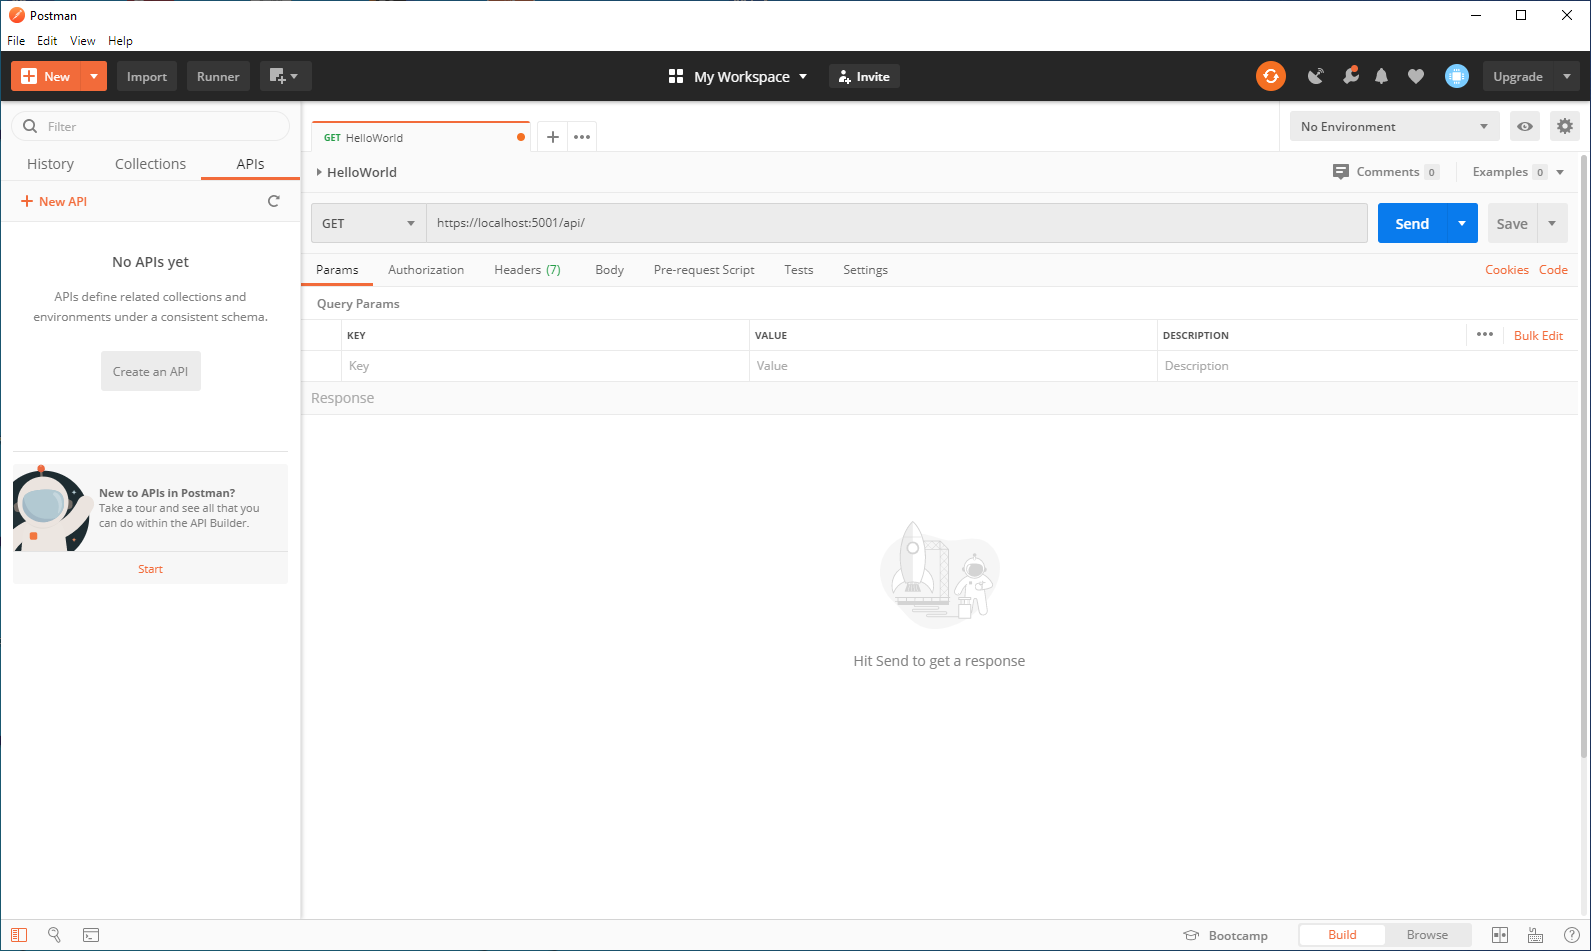
\includegraphics[width=1\textwidth, frame]{./grafiken/postman.png}
	}
	\vskip0pt
	\caption{UI von Postman} \label{fig:postman}
\end{figure}


\section{JSON Web Token}
JSON Web Token(JWT) ist ein Access-Token, der auf JSON basiert. Durch JWT kann man verifizierbare Claims austauschen. Mit JWT sind Stateless Sessions möglich, da jede benötigte Information für eine Authentifikation mit dem Token übertragen werden kann. Ein JSON Web Token setzt sich aus dem Header, Payload und der Signatur zusammen. Bei einem Request mit einem Token schreibt man vor dem Token noch "Bearer". \autocite{wikiJWT}

Der Header ist ein JSON-Element. Darin ist gespeichert, welcher Token-Typ es ist und welche Verschlüsselungsmethode angewendet wird. Der Typ ist JWT und als Verschlüsselungsmethoden wird meist HMAC mit SHA-256 oder RSA mit SHA-256 verwendet. \autocite{wikiJWT} \\
\begin{lstlisting}[caption={JWT-Header Beispiel}, language=json]
	{
		"alg": "HS256",
		"typ": "JWT"
	}
\end{lstlisting}

Der Payload ist ebenfalls ein JSON-Element. In diesem JSON sind die Claims beschrieben. Es gibt einige reservierte Claims, die den Aussteller, das Subject oder das Ablaufdatum beschreiben, jedoch kann der Aussteller auch einen Private Claim definieren. \autocite{wikiJWT} \\
\begin{lstlisting}[caption={JWT-Payload Beispiel}, language=json]
	{
		"sub": "8135731594",
		"name": "Max Mustermann",
		"admin": true
	}
\end{lstlisting}

Durch JSON Web Signature(JWS) wird die Signature definiert. Die ist nach RFC 7515 genormt. Mit der im Header festgelegten Hashmethode wir der Header und der Payload Base64 kodierten und durch einem Punkt-getrenntem Format gehasht. Das Ergebnis ist die Signature. \autocite{wikiJWT}

Der JWT-Token setzt sich nun aus dem jeweils Base64-Url kodierten Header, Payload und Signature mit einem Punkt getrennt zusammen. \autocite{wikiJWT} \\
Der Nachfolgende Token setzt sich aus den zwei Beispielen zusammen:\\
\texttt{
	eyJhbGciOiJIUzI1NiIsInR5cCI6IkpXVCJ9.eyJzdWIiOiI4MTM1NzMxNTk0IiwibmFtZSI6I\\k1heCBNdXN0ZXJtYW5uIiwiYWRtaW4iOnRydWV9.8NyZnCtWX\_QAlNhfl70zD2tHR\\9j1mtSl9Dwdfnnh60k
}

\section{Google Maps Place Autocomplete}

Der Dienst "Place Autocomplete" ist ein Webdienst, der als Antwort auf eine HTTP-Anfrage Ortsvorhersagen zurückgibt. Die Anfrage gibt einen textuellen Suchstring und optionale geografische Grenzen an. Der Dienst kann verwendet werden, um eine Autovervollständigungsfunktion für textbasierte geografische Suchen bereitzustellen, indem Orte wie Unternehmen, Adressen und Points of Interest zurückgegeben werden, während ein Benutzer sie eingibt.\cite{googlePlacesAPI}

Der Dienst "Place Autocomplete" kann ganze Wörter und Teilstrings abgleichen und so Ortsnamen, Adressen und Pluscodes auflösen. Anwendungen können daher Abfragen senden, während der Benutzer tippt, um on-the-fly Ortsvorhersagen zu erhalten.Die zurückgegebenen Vorhersagen sollen dem Benutzer bei der Auswahl des gewünschten Ortes helfen. Sie können eine Abfrage für Ortsdetails senden, um weitere Informationen über jeden der zurückgegebenen Orte zu erhalten.\cite{googlePlacesAPI}

\section{Shopify}
Das Node-Package "@shopify/address" liefert für die Länder die verpflichtenden Felder und falls vorhanden die Staaten oder Provinzen für eine gültige Adresse durch die Methode \texttt{getCountry(countryCode)}. Dadurch ist es möglich, dass an das jeweilig ausgewählte Land, die Pflichtfelder angepasst werden. Durch die Methode \texttt{getOrderedFields(countryCode)} erhält man die richtige Reihenfolge eines Formulars für das Land. Das Resultat dieser Abfrage ist eine zweidimensionales Array, woraus man den Inhalt der einzelnen Zeilen herauslesen kann. Der Parameter "countryCode" steht für die internationale Länderabkürzung, in Falle Österreich wäre dieser "AT". \autocite{shopifyNPM}

\section{Twilio} \label{sec:twilio}
Twilio wurde 2008 von Jeff Lawson, Evan Cooke und John Wolthuis in Amerika gegründet. Es betreibt eine Cloud-Kommunikationsplattform als Platform as a Service. Mit den von Twilio zur Verfügung gestellten Dienst, können Entwickler Programmierschnittstellen zum ausführen und empfangen von Anrufen, senden von SMS, verifizieren von Telefonnummern sowie für andere Kommunikationsfunktionen nutzen. In unseren Implementationen half Twilio bei der Verifizierung der von den Benutzer angegebenen Telefonnummern. \cite{twilioWebsite}

\section{Address Validator}
Der Address Validator wurde von Byteplant Software Solutions \& Services entwickelt. Dieses Unternehmen wurde 2003 in Deutschland gegründet. Neben dem Address Validator bieten sie auch einen Email Validator und einen Phone Validator an. Die Adressvalidierung hilft dabei, Informationen über die Zustellbarkeit einer Adresse zu sammeln, Korrekturvorschläge zu präsentieren, falls die Adresse nicht ganz gültig ist und eine einheitliche Adressformatierung nach den nationalen Standards anzubieten. Für eine Überprüfung benötigt man Straße, Stadt, Internationales Länderkürzel und den API-Key. Optional kann man noch mehr, wie beispielsweise Postleitzahl oder die Locale in der man das Ergebnis erhalten möchte, validieren. Als Antwort bekommt man eine Datei im JSON-Format. Aus dieser JSON-Datei ist es möglich, viele Informationen über die Adresse auszulesen. Falls die Adresse gültig ist, bekommt man im Feld Status ein VALID, bei ungültiger Adresse ein INVALID und falls die Überprüfung kein genaues Ergebnis herausgefunden hat, aber eine Adresse gefunden hat, die es sein könnte, ist der Status SUSPECT mit einen Adressvorschlag. Weiteres beinhaltet die Antwort alles von den einzelnen Adressfelder bis hin zu der formatierten Adresse des Landes und den Geografischen Koordinaten. \cite{addressValidator}

\section{Google Translator}
Die Schnittstelle für den Google Cloud Translator wurde von Google LLC entwickelt. Damit kann man schnell Texte in mehr als 100 Sprachen im eigenen Programm übersetzen lassen. Als Antwort der Übersetzung bekommt man den Titel, den Inhalt und die Abkürzung der Sprache. Nun kann man die Übersetzungen speichern und man braucht nur nach der Spachenabkürzung suchen.
\cite{googleTranslator}

\section{Auth0}
Auth0 wurde 2013 gegründet. Der Hauptsitz dieses Unternehmen liegt in Bellevue, Amerika. Mit Auth0 können die Authentifizierungs- und Autorisierungsfunktionen ausgelagert werden. Im Hintergrund von dieser Identitätsmanagement Lösung gibt es die Möglichkeit, dass mehrere Datenquellen zum Anmelden verwendet werden können. \autocite{auth0}

\section{zxcvbn}
Um die Passwortstärke herauszufinden, wurde zxcvbn verwendet. Es erkennt und bewertet Passwörter durch Musterabgleich, Vergleich mit häufige Namen und Nachnamen, englische Wörter aus Wikipedia, Fernsehshows und Filme und Wiederholungen und Tastaturmuster. Als Antwort bekommt man Informationen, wie sicher das Passwort ist und ein Feedback mit einer Warnung und einem Tipp, wie man es noch sicherer machen könnte. \autocite{zxcvbn}